%%% start preambling . . .  %%%
\documentclass{article}

% required 
\usepackage{amsmath}
\usepackage{natbib}
\bibliographystyle{plainnat} %{unsrtnat}
\usepackage{xr-hyper}
\usepackage{hyperref}
\externaldocument[supplement-]{supplement}
\usepackage{booktabs,siunitx}
\usepackage{Sweave}
\usepackage{graphicx}
\usepackage{lipsum}                     % Dummytext % https://tex.stackexchange.com/questions/9796/how-to-add-todo-notes
\usepackage{xargs}                      % Use more than one optional parameter in a new commands
\usepackage[pdftex,dvipsnames]{xcolor}  % Coloured text etc.

\usepackage[colorinlistoftodos,prependcaption,textsize=tiny]{todonotes}
\newcommandx{\unsure}[2][1=]{\todo[linecolor=red,backgroundcolor=red!25,bordercolor=red,#1]{#2}}
\newcommandx{\change}[2][1=]{\todo[linecolor=blue,backgroundcolor=blue!25,bordercolor=blue,#1]{#2}}
\newcommandx{\info}[2][1=]{\todo[linecolor=OliveGreen,backgroundcolor=OliveGreen!25,bordercolor=OliveGreen,#1]{#2}}
\newcommandx{\improvement}[2][1=]{\todo[linecolor=Plum,backgroundcolor=Plum!25,bordercolor=Plum,#1]{#2}}
\newcommandx{\thiswillnotshow}[2][1=]{\todo[disable,#1]{#2}}


% https://tex.stackexchange.com/questions/60209/how-to-add-an-extra-level-of-sections-with-headings-below-subsubsection
\usepackage{titlesec}
\setcounter{secnumdepth}{4}

\titleformat{\paragraph}
{\normalfont\normalsize\bfseries}{\theparagraph}{1em}{}
\titlespacing*{\paragraph}
{0pt}{3.25ex plus 1ex minus .2ex}{1.5ex plus .2ex}



% recommended! Uncomment the below line and change the path for your computer!
 
%put your figures in one place! Also, note that here 'figures' is the folder and 'demoFig' is what each 
% figure produced will be titled plus its number or label (e.g., demoFig-nqpbetter.pdf')

% make your captioning look better
\usepackage[small]{caption}
\setlength{\captionmargin}{30pt}
\setlength{\abovecaptionskip}{0pt}
\setlength{\belowcaptionskip}{10pt}

% optional: muck with spacing
\topmargin -1.5cm        
\oddsidemargin 0.5cm   
\evensidemargin 0.5cm  % same as oddsidemargin but for left-hand pages
\textwidth 15.59cm
\textheight 21.94cm 
% \renewcommand{\baselinestretch}{1.5} % 1.5 lines between lines
\parindent 0pt		  % sets leading space for paragraphs
% optional: cute, fancy headers
\usepackage{fancyhdr}
\pagestyle{fancy}
\fancyhead[LO]{November 2022}
\fancyhead[RO]{Manuscript}
% more optionals! %
% \usepackage[hyphens]{url} % this wraps my URL versus letting it spill across the page, a bad habit LaTeX has
%%% end preambling. %%%

\begin{document}
\Sconcordance{concordance:supplement.tex:supplement.Rnw:%
1 65 1}
 % For RStudio hiccups
\title{{\huge Changes and trends in budburst and leaf flush across Europe and North America} \\A meta-analysis of local adaptation in spring phenology studies}
\author{Ziyun Zeng \& E. M. Wolkovich}
\date{November 2022}
\maketitle 


\newpage

\section*{Abstract}


We conducted the first cross-continental meta-analysis of published studies from the peer-reviewed literature that reported spring event dates for a mix of angiosperm and gymnosperm tree species in the northern hemisphere, capturing data from 384 North American provenances and 101 European provenances with observations from 1962 to 2019.


\section{Introduction}
\begin{itemize}
\item Define spring event, fall event
\item Background
\item Importance: An accurate understanding of how species distribution might be influenced by environmental conditions at a continental scale is critical for future range shift prediction. 
\item Knowledge Gap: Anecdotally, the spring phenology of trees from European provenances appeared to exhibit stronger clines and less plasticity than in North American studies. Despite a growing interest in predicting local adaptation across locations, no study has comprehensively examined clines for spring and fall events and what factors may underlie differences observed across studies.
\item Research question (links to results)
\end{itemize}

We ask: Across common garden studies, how strong are clines in spring and fall phenology?

To better understand these clines, we also aim to examine:
\begin{itemize}
\item If differences in clines exist across Europe and North America.
\item If differences in clines exist across angiosperm and gymnosperm species.
\item If climate overlap (see Figure 1) between the provenance and garden explains the similarities and differences in clines.
\end{itemize}
To our knowledge, this marks the first study to synthesize spring phenology data retrieved from studies across North America and Europe. 


\subsection*{Ref notes}
\todo[inline]{Good background information.}

\citep{AitkenBemmels16}\\
"Geographic variation in trees has been investigated since the mid-18th century. Similar patterns of clinal variation have been observed along latitudinal and elevational gradients in common garden experiments for many temperate and boreal species."\\
"Scientists have studied relationships between tree populations and environmental characteristics of their provenances in common garden experiments for over 250 years."\\
\\
\citep{Alberto13}\\
"Evolutionary responses are required for tree populations to be able to track climate change. Results of 250 years of common garden experiments show that most forest trees have evolved local adaptation, as evidenced by the adaptive differentiation of populations in quantitative traits, reflecting environmental conditions of population origins."\\
"Thus, responding to climate change will likely require that the quantitative traits of populations again match their environments. We examine what kind of information is needed for evaluating the potential to respond, and what information is already available. We review the genetic models related to selection responses, and what is known currently about the genetic basis of the traits. We address special problems to be found at the range margins, and highlight the need for more modeling to understand specific issues at southern and northern margins. We need new common garden experiments for less known species. "\\
"Modeling work on the potential of populations and species to respond genetically to recent climate change is advancing (see Hoffmann \& Sgrò, 2011; Franks \& Hoffmann, 2012; Shaw \& Etterson, 2012 for recent reviews). "\\

(see e.g., Valladares et al., 2007; Caffarra et al., 2011; Hänninen \& Tanino, 2011)
"The plastic response of different traits (e.g., phenology in trees) to variation in climate is, however, often much more complex than in heuristic models of adaptation."\\


\citep{Loarie09}\\ 
"It is also now understood that the rate of adaptation required by climate change varies among geographic regions." \improvement{need to read again}\\

\citep{Nicotra10}\\ 
"The immediate responses via phenotypic plasticity have also been considered in the context of climate change." \improvement{need to read again}\\

\citep{Menzel99} \textbf{Growing season extended in Europe.}\improvement{good Europe background paper}\\
\citep{Menzel06} \textbf{European phenological response to climate change matches the warming pattern.}\improvement{another good Europe background paper}\\
\citep{Parmesan06}\\
"Trees exhibit a high degree of phenotypic plasticity with respect to climatic variation. Phenological shifts of bud flush in response to recent increases in temperatures have been widely documented ." \improvement{can cite more papers on this matter}


\citep{Gill15} \textbf{Changes in autumn senescence in northern hemisphere deciduous trees: a meta-analysis of autumn phenology studies.} \improvement{GREAT paper for us to base our writing on: similar meta-analysis but focuses on fall events}\\
"the effects of climate change on the phenology of vegetation have received increased attention over the past several decades as any factor that alters the timing of early growing season leaf-out and senescence has the potential to affect a variety of ecosystem properties. For example, the timing of leaf-out and senescence of deciduous plants has been shown to affect plant competition (Fridley, 2012), plant growth (Myneni et al., 1997) and ecosystem carbon uptake (Barichivich et al., 2012).\\

"While leaf-out has been shown to advance over the past century as a result of increasing air temperatures (Linderholm, 2006; Polgar and Primack, 2011), the relationship between temperature and leaf senescence remains less well understood (García-Plazaola et al., 2003; Richardson et al., 2013)."

"Thus, an extension of the growing season can contribute to reduced atmospheric CO2 concentrations due to enhanced carbon sequestration in terrestrial plants (Penuelas et al., 2009; Richardson et al., 2013). However, the increase in carbon uptake may be partially offset by increased rates of ecosystem respiration (Piao et al., 2008)"

"The lack of consistent relationships between air temperature and timing of leaf senescence suggests that autumn senescence may be influenced by a variety of factors that obscure its relationship with temperature."


\todo[inline]{Cite some papers about the documented trends}

tbc...

 
 

\todo[inline]{Alina says: I found AitkenBemmels2016's research question to be wonderfully phrased and think we can do something similar}
\citep{AitkenBemmels16}\\
"To what extent are patterns of local adaptation along climatic gradients similar among species within a given geographic region? If clines in phenotypic traits are similar, can average patterns of sympatric variation guide AGF or identify critical climatic variables as a first approximation for untested species? We reanalysed data from the literature on provenance trials in temperate tree species from western North America to address these questions. This is an ideal region of focus because of the many provenance trials conducted on native tree species that are important for forestry, and because its high topographic complexity means that turnover in climate occurs rapidly and heterogeneously over short geographic spaces. Clines along climate gradients are thus espcially likely to reflect local adaptation to climate, rather than non-adaptive phenomena resulting from population demographic history."
 




\section{Methods}
Our methods are divided into four main steps. 

% \item Literature search
\subsection{Literature Search}

We searched the peer-reviewed literature for common garden experiments that documented the timing of spring events of woody plant species. We searched on the Web of Science (Thompson Reuters, New York, NY) using all combinations of the following terms as ‘titles’ including ‘common garden*’ or “provenance*’ and ‘leafout*’ or ‘leaf out*’ or ‘budburst’ or ‘spring phenolog*’. Our search was limited to journal articles published before November 3, 2021. The search returned 94 publications. 
\\

\todo[inline]{question for lizzie: I later checked 2022 publications too to make sure we didn't miss anything... Do I just say at the very beginning that our search is limited to publications before Dec 14, 2022, or do I say 'we later checked the literature again on XX-XX-2022 to ensure we did not miss any new publications?}
\todo[inline]{I also think the reviewers might question why we had so few search results.... maybe I should mention that I also checked on Google Scholar and Connected Papers, and Aitken Bammals 2016/Alberto 2013, and emailed our list of papers to established researchers such as Aitken and Guy, etc. to make sure we didn't miss anything?}

We read the methods and results of all publications returned and limited our subsequent analysis to the ones that (a) focused on woody plants originating from either Europe or North America, (b) had provenance trails and common gardens on the same continent, (c) reported spring events in units of calendar days (day of year or DOY) instead of a quantitative scale on a particular day, and (d) reported latitude and longitude of provenances and gardens. 
\\
We had to exclude studies that reported spring events on a quantitative scale because (1) such studies usually only assessed where on the scale the spring event of a tree fell onto on the same days across different years (e.g. Robson et al., 2013; Vander et al., 2015; Santini et al., 2014; Schueler \& Liesebach, 2004), and (2) scales are not always consistent across different studies (Chmura \& Rozkowski 2002; Dhont et al., 2010; Wang et al., 2022). Such factors made it impossible to back convert the quantitative scale to DOY.
\todo[inline]{add these citations to bibtex?? do we cite them?}

Some studies did not provide the exact latitude and longitude of the common garden (Bongarten, 1978) or the provenances (Hall et al., 2007; Soolanayakanahally et al., 2013), or they did not link the latitude and longitude of each provenance to the DOY of spring events (Deans \& Harvey, 1996). We had to exclude these papers. We also left out studies in which woody plants from North American provenances were planted in common gardens in Europe because we wanted to test continental variations (Cannell et al., 1987; Lavadinovic et al., 2013). Finally, we excluded studies that focused on examining how provenance altitude influenced local adaptation in spring phenology since we are interested in testing latitudinal effects (Vitasse et al., 2009; Vitasse et al., 2010; Li et al., 1997; Alberto et al., 2011; Acevedo-Rodríguez et al., 2006). 

% Read AB 2015 and A 2013 for anything that we missed, took paper with spring doy and provenance coordinates from them 

\subsection{Dataset Assembly}

Out of XX papers related to common garden/spring phenology that we read, only 18 (?) ultimately supplied the data that we needed (DOY of spring events, latitude and longitude of provenances and common gardens). \improvement{need to rewrite this; can display a table here} Studies were distributed throughout North America and Europe, with the majority of data concentrated in XXXXX (Figure X). The distribution was skewed toward North America (n = X), with only X located in Europe. We primarily focused our analysis on spring events, and made use of the fall event DOYs present in X of the studies we included rather than searching for publications entirely on fall events online. 
\\
% We retained studies that supplied DOY of spring events and geographic coordinates of provenances and common gardens. 

We assembled a data set that documents event DOY and geographic coordinates of provenances and gardens, during which we used ImageJ (version 1.53k; Rasband, 1997-2022) to extract values from figures whenever possible and necessary. We pooled the timing of budburst and leaf flush into a single category of ‘spring events’ and the timing of bud set, leaf senescence, growth cessation, and leaf abscission into ‘fall events.’ Such pooling is justified because of the shared pressures from natural selection that govern these events (Gill et al., 2015). Some studies documented event dates relative to a reference date that is not January 1 (e.g. Cannel et al., 1987; Rehfeldt, 1994). In this case, we converted such dates to DOY using the Lubridate Package in R for standardization purposes.
\\


Some studies had more than one gardens (), two studies shared the same garden ().\improvement{can mention this in table caption}

Most common garden studies that supplied data only had observations of one tree species, which makes it difficult for a model to interpret if variations across gardens are due to the species or the garden’s location and climate. We thus focused on estimating species effects because we expect a larger effect from species. Within publications, we considered unique gardens and species to represent independent data, and fitted each species \& common gardens instead of just species. \improvement{need to phrase this better, and maybe put this somewhere in the modelling methods}



\subsection{Climate Data Gathering \& Analyses}
  \begin{itemize}
  \item Simple climate matrix (MAT \& MSP/MAP) gathering
  \begin{itemize}
  \item ClimateNA by Dr. Tongli Wang
  \item Climate Information Tool by FAO
  \end{itemize}
  \item Daily climate data gathering: Gridded daily climate data downloaded for all provenances and gardens: We hope that coarse metrics such as latitude and MAT ultimately represent how similar the climates are between the provenances and gardens in times that matter for the events. If climates are very similar, then we would expect similar timings [add more here].
To this end, we estimated climate overlap in relevant months: For spring events, we considered overlap across March to May.
  \begin{itemize}
  \item North American daily climate data from Daymet R package
  \item Europe daily climate data (gridded: NetCDF-4) retrieved from E-OBS 
  \end{itemize}
  \end{itemize}

\subsubsection{Estimate climate overlap using daily climate data using Overlap R package}
\subsubsection{Calculate GDDs}


Growing degree days (GDD) is a commonly used heat accumulation measure to forecast phenological development in plants (Miller et al., 2001). We calculated GDD based on the accumulation of mean daily temperatures ($T_{m}$)from 2011 to 2022 above a baseline of 0$^{\circ}$C, from January 1 until budburst and leaf flush with the following formula: GDD = $\sum$($T_{m}$ - $0^{\circ}$C for $T_{m}$ $\ge$ $0^{\circ}$C; 0 for $T_{m}$ $\le$ $0^{\circ}$C) 


\subsubsection{Spherical distances}



\subsubsection{Corrected for DOY (taking the difference)}\todo{will put results in supplement}
\subsection{Mixed effects modelling}

We used hierarchical Bayesian models where we partially pooled by species. We estimated effects of continent and species type (angiosperm VS gymnosperm) from posterior estimates, in relation to single predictors (including provenance latitude, MAT) and two predictors (climate overlap percentage and standard deviation). \improvement{will elaborate later}


\section{Results}

\verb@Research questions recap@
\\
Despite a growing interest in predicting local adaptation across locations, no study has comprehensively examined clines for spring and fall events and what factors may underlie differences observed across studies.

We ask: Across common garden studies, how strong are clines in spring and fall phenology?

To better understand these clines, we also aim to examine:
\begin{itemize}
\item If differences in clines exist across Europe and North America.
\item If differences in clines exist across angiosperm and gymnosperm species.
\item If climate overlap between the provenance and garden explains the similarities and differences in clines.
\end{itemize}

\todo[inline]{all subsection titles are placeholders}
Out of the X papers on common garden experiments and spring phenology that we reviewed, only 18(?) supplied data met our criteria to be included: (a) focus on woody plants originating from either Europe or North America, (b) report spring event in units of calendar days instead of a quantitative scale on a particular day, (c) report locations of provenances and gardens. 

% Out of the 22, four studies had provenances and common gardens on different continents. These studies were excluded from our main analysis, but we document them in our supplements.\change{need to reword}
Our final dataset captures seven angiosperm and eight gymnosperm species from 19 common gardens, encompassing data from 384 North American provenances and 101 European provenances with observations from 1962 to 2019. Seven species had fall event information available. 
\\
It is worth noting that most common gardens included in this study only had observations of one species. Therefore, it is difficult for a model to interpret if variations across gardens are due to the species or the garden’s location and climate. \improvement{can refer to the fit we did where we fitted each species \& common garden instead of just species} We thus focused on estimating species effects because we expect a larger effect from species. 

\todo[inline]{add map here}
\todo[inline]{add a table documenting studies attributes}

\subsection{Provenance latitude and MAT do not affect spring event timing}

Overall, our models show that spring events are not related to provenance latitude or mean annual temperature in North America, and only weakly related in Europe (Fig. \ref{figure:springfall_latmat} \& Supplement Table.\ref{supplement-table:model_sf_lat}). \unsure{Should I add climate overlap plots here too?}


\begin{figure}[!h] 
    \centering
 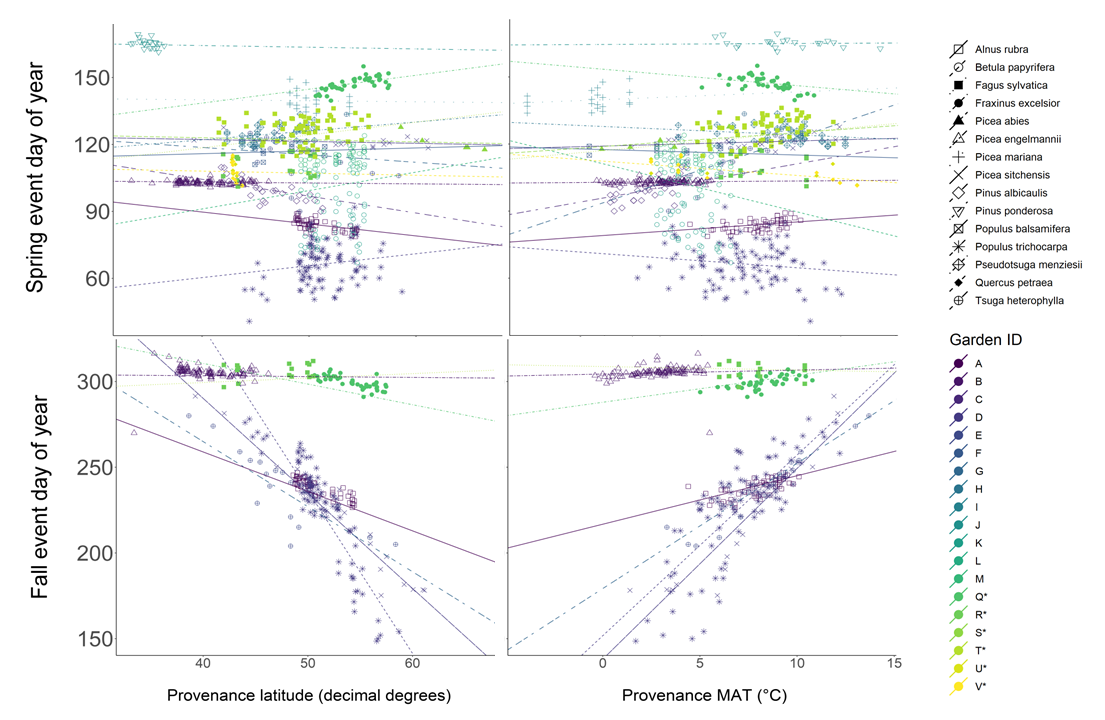
\includegraphics[width=\textwidth]{..//..//localadaptclim/Docs/figure_ms/springfall_latmat.png}
    \caption{Spring event Day of Year (DOY) in relation to provenance latitude and MAT, coded by symbol for species and color for garden with linear fits from hierarchical Bayesian models. Spring events shown on top and fall event at the bottom.}
    \label{figure:springfall_latmat}
\end{figure}


\newpage

\subsubsection {Similar results across provenance latitude, latitude difference, and distance}
\todo[inline]{need to find a name for each metric and stick to it.}
Along with (a) provenance latitude, we also looked at how spring event timing is related to (b) the absolute difference between provenance latitude and garden latitude , as well as (c) the spherical distance between the garden and each provenance. All three metrics depict little to no relationship between spring event timing and the geographical location of the provenance (Supplement Fig.\ref{supplement-figure:lat_distance}).

\newpage
\subsubsection {Climate overlap does not predict event dates much better than provenance latitude or MAT}

While comparing how similarity in climate relates to event dates, we observed very weak effects of climate overlap on spring events, nearly identical across angiosperms and gymnosperms. Fall events diverge as climate overlap declines for both angiosperms and gymnosperms, but slightly more strongly for gymnosperms (Fig.\ref{figure:overlap}).

\begin{figure}[!h] 
    \centering
 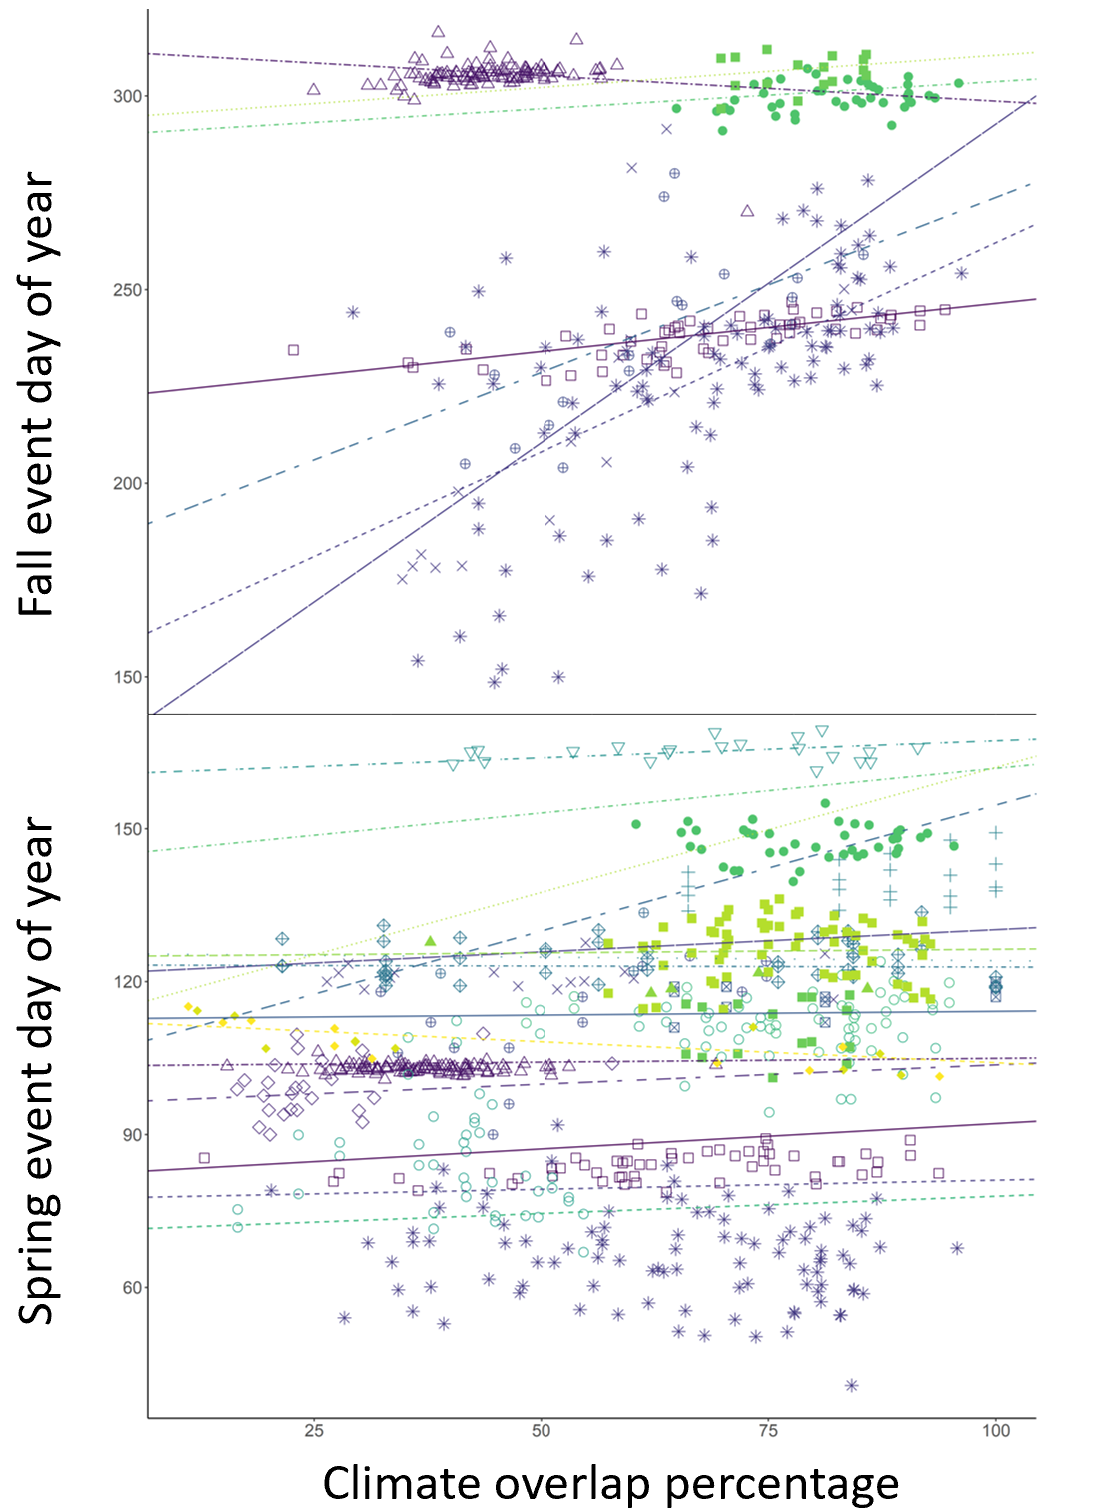
\includegraphics[width=\textwidth]{..//..//localadaptclim/Docs/figure_ms/climate_overlap.png}
    \caption{Caption placeholder}
    \label{figure:overlap}
\end{figure}


\subsection{Stronger clines in fall events observed in North America than Europe}

% old graphs can be found in C:\Users\alina\Documents\git\localadaptclim\Output\plotMay15_two predictors_experiment
% refer to analyses\script_model_continent_spp_type_effect
% https://github.com/lizzieinvancouver/localadaptclim/issues/16

% need to replot ofc


%  extract the mean estimate of the slope and report that instead of ~4 or such
% hmmm i forgot the code :)))

We find that fall events (budset, leaf senescence, leaf abcission) advance strongly with provenance latitude and mean annual temperature, meaning fall events are earlier where provenance mean annual temperature is lower (higher, more northern latitudes). This relationship, however, is observed mostly in North America where fall events advance 4.2 days per degree we move north, or 6.4 days when the MAT decreases by 1 $^{\circ}$C (Fig. \ref{figure:continent}). In Europe, such relationship is weak: advance 0.5 days per degree we move north, or 0.6 days when the MAT decreases by 1 $^{\circ}$C(Fig. \ref{figure:continent}).

\begin{figure}[!h] 
    \centering
 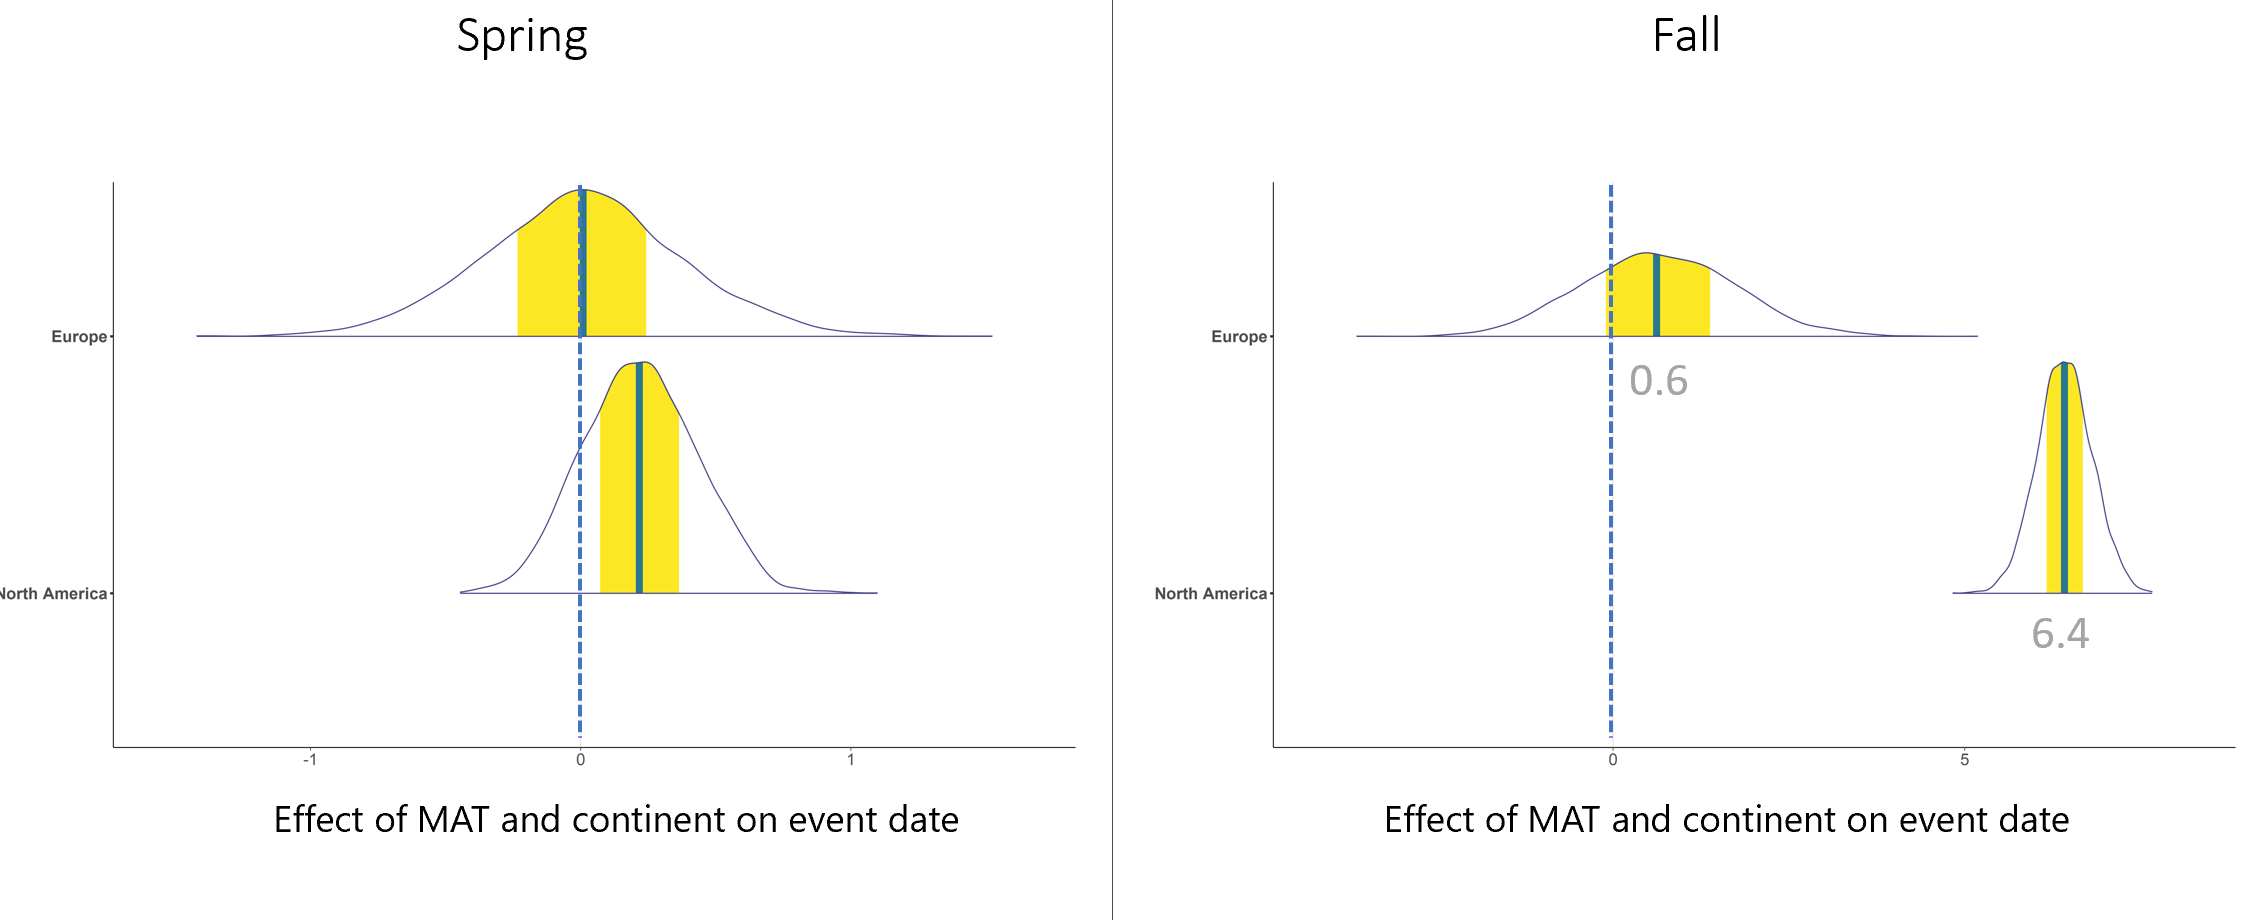
\includegraphics[width=\textwidth]{..//..//localadaptclim/Docs/figure_ms/continent_histogram.png}
    \caption{Caption placeholder}
    \label{figure:continent}
\end{figure}


\subsection{Effects of MAT on spring events diverge across angiosperms and gymnosperms}

Effects of provenance latitude on both spring and fall events are similar across angiosperms and gymnosperms. However, effects of MAT on spring events weakly diverge: spring events get earlier as MAT increases in angiosperms and delay as MAT increases in gymnosperms, except for \emph{Pseudotsuga menziesii}. Fall events delay in warmer locations for both species types, but slightly more so for gymnosperms (3.7 days VS. 6.2 days)(Fig. \ref{figure:spp_type}).

\begin{figure}[!h] 
    \centering
 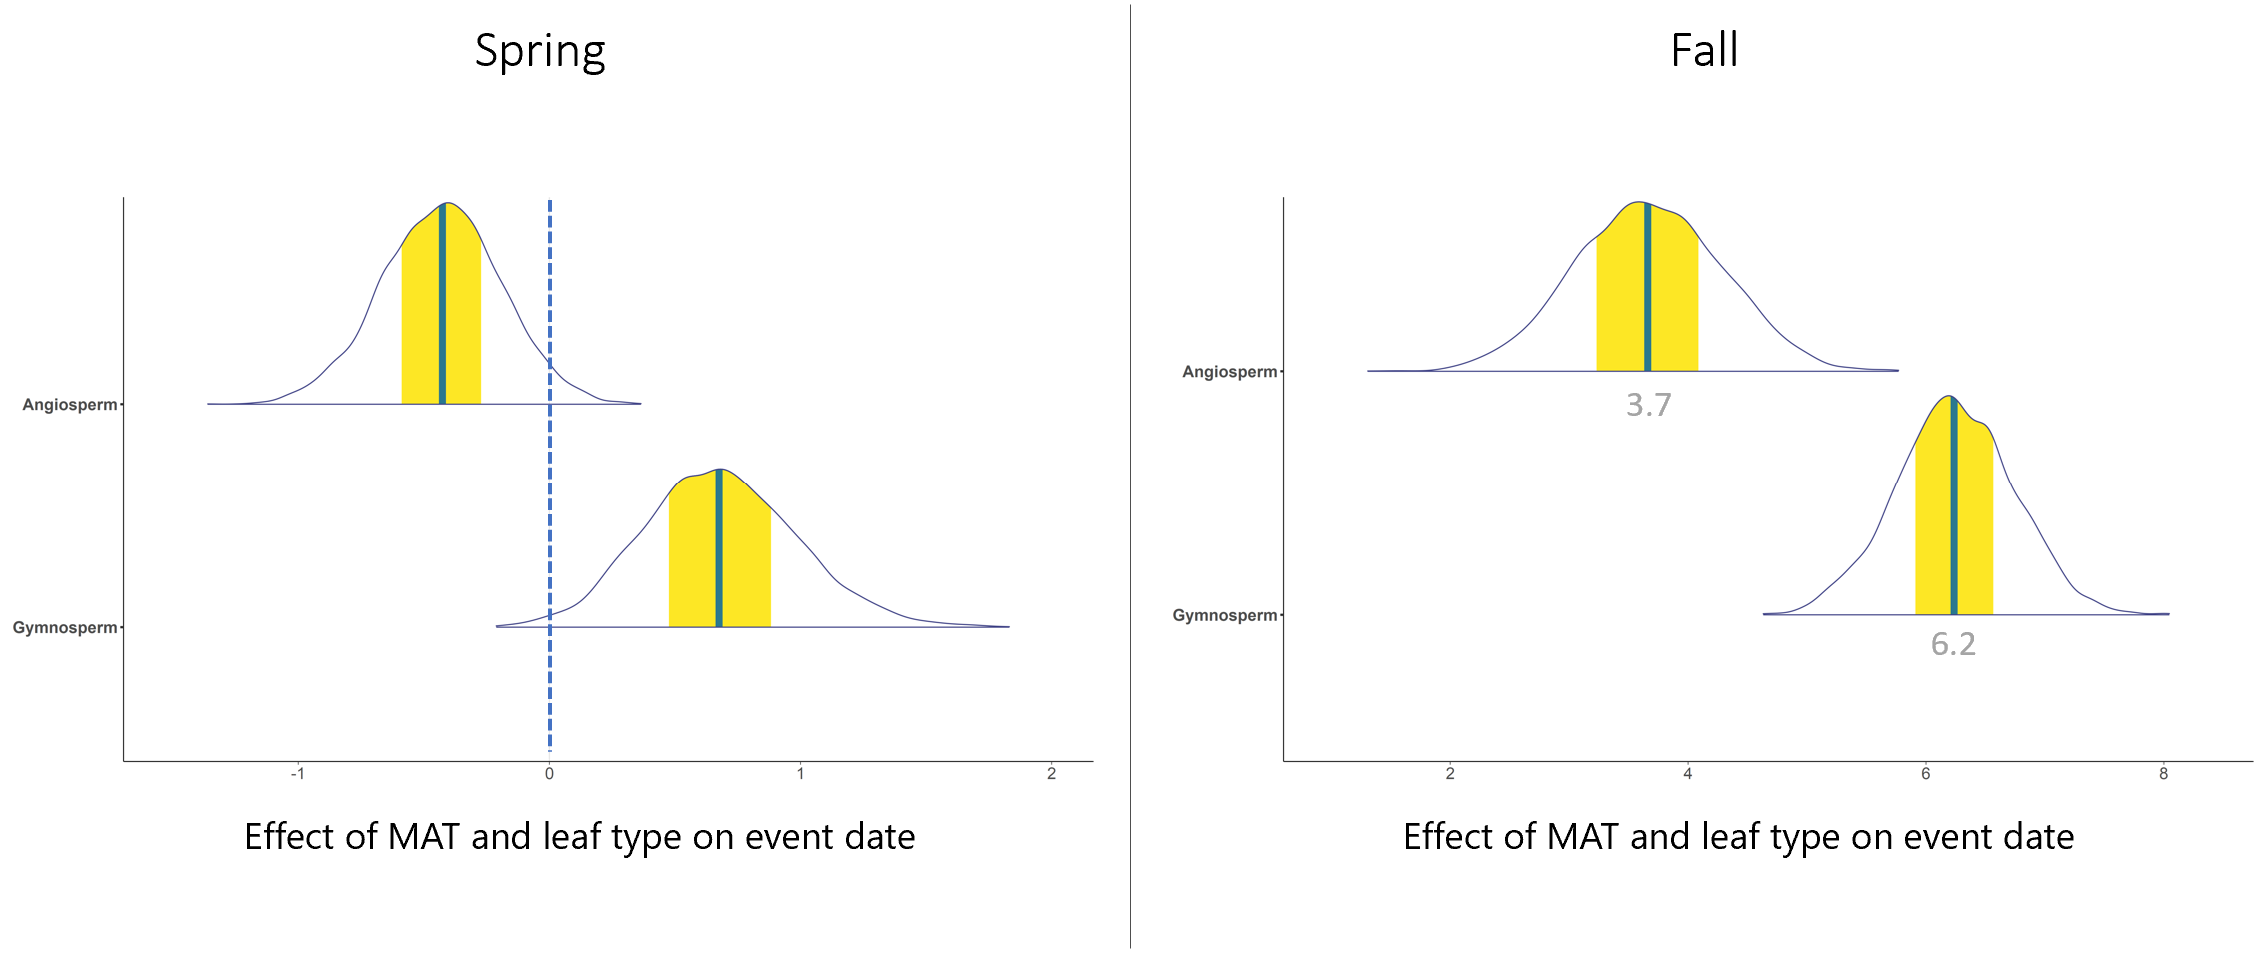
\includegraphics[width=\textwidth]{..//..//localadaptclim/Docs/figure_ms/spp_type_histogram.png}
    \caption{Caption placeholder}
    \label{figure:spp_type}
\end{figure}


\section{Discussion}




The weak relationship between spring event dates and provenance latitude and MAT that we find in European studies might be explained by the higher extent of climate overlap in those studies. The more similar the climate is between provenances and gardens, the less difference between spring event dates.
\\

The inconsistent and weak clines in spring events that we found suggest high plasticity in spring phenology across continents and species. Fall events, on the other hand, exhibit stronger clines which suggest more local adaptation, especially in North America. Overall, our results predict that warming springs will continue to be tracked more closely phenologically by trees than warming fall temperatures.
\\

In contrast to spring events, we found strong latitudinal clines in fall events across both continents, with local adaptation appearing much stronger in North America than in Europe. Our results show that spring events are highly plastic, and thus may shift with warming, but data on more species and greater information on important factors, such as their geographic location in relation to their origins and elevation, are needed for forecasting. 






\citet{Keir11}



\section{Figures}


Rasband, W.S. (1997-2016). Image J.U.S. National Institute of Health, Bethesda, Maryland, USA.
http://imagej.nih.gov/ij

\bibliography{bibliography_local_adaptation.bib}






\end{document}




% helping with abstract language
% Alberto16
% "On the basis of the patterns of quantitative variation for 19 adaptation-related traits studied in 59 tree species (mostly temperate and boreal species from the Northern hemisphere), we found that genetic differentiation between populations and clinal variation along environmental gradients were very common (respectively, 90% and 78% of cases)."

% formatting code resources
% https://github.com/lizzieinvancouver/ospree/blob/master/docs/ranges/ranges_outline.tex
% https://github.com/lizzieinvancouver/ospree/blob/master/docs/traits/Traitors_Manuscript_supp.Rnw

